% =============================================================================
%  manuscript.tex
%  Draft submission to Computers & Geosciences (Elsevier)
%
%  Compile from this directory:
%      ./compile.sh manuscript.tex
% =============================================================================

% --- elsarticle alternative (uncomment when ready to submit) -----------------
% \documentclass[review,12pt,authoryear]{elsarticle}
% \journal{Computers \& Geosciences}
% -----------------------------------------------------------------------------
\documentclass[11pt,a4paper]{article}

\usepackage[a4paper,margin=2.5cm]{geometry}
\usepackage{lineno}
\usepackage[colorlinks=true,linkcolor=blue!50!black,citecolor=blue!40!black,urlcolor=blue!50!black]{hyperref}
\usepackage{graphicx}
\usepackage{amsmath,amssymb}
\usepackage{booktabs}
\usepackage{xcolor}
\usepackage{listings}
\usepackage{enumitem}
\usepackage{microtype}
\usepackage{authblk}
\usepackage[super,sort&compress,comma]{natbib}
\usepackage{algorithm}
\usepackage{algpseudocode}
\usepackage{dblfloatfix}   % allow figure*/table* at the bottom of a page
\usepackage{quantikz}
\usepackage{makecell}
\usepackage{tikz}
\usepackage{orcidlink}
\usetikzlibrary{arrows.meta, fit, backgrounds, shapes.geometric}

% Looser float-placement parameters so figures don't get pushed pages away.
\renewcommand{\topfraction}{0.95}
\renewcommand{\bottomfraction}{0.95}
\renewcommand{\textfraction}{0.05}
\renewcommand{\floatpagefraction}{0.7}
\renewcommand{\dbltopfraction}{0.95}
\renewcommand{\dblfloatpagefraction}{0.7}
\setcounter{topnumber}{3}
\setcounter{bottomnumber}{3}
\setcounter{totalnumber}{6}
\setcounter{dbltopnumber}{3}

\renewcommand{\Authfont}{\bfseries}
\renewcommand{\Affilfont}{\mdseries\normalfont\small}
\setlength{\affilsep}{0.4em}

\modulolinenumbers[5]

% Expose the internal @twocolumnfalse environment so the title/abstract can
% span both columns via \twocolumn[\begin{strip}...\end{strip}].
\makeatletter
\newenvironment{strip}{\begin{@twocolumnfalse}}{\end{@twocolumnfalse}}
\makeatother

\definecolor{todoRed}{RGB}{180,30,30}
\newcommand{\todonote}[1]{\textcolor{todoRed}{\textbf{[TODO: #1]}}}
\newcommand{\needs}[1]{\textcolor{todoRed}{\textbf{[NEEDED: #1]}}}
% Mark newly-introduced citations so the author can vet them against the
% curated refs.bib.  Usage: \newcite{Smith2020}.
\newcommand{\newcite}[1]{\textcolor{todoRed}{$^{\ast}$}\citep{#1}}

% Drop-in replacements for elsarticle's frontmatter / highlights / keyword envs
\newenvironment{frontmatter}{}{}
\newenvironment{highlights}{%
  \begin{quote}\textbf{Highlights}\par\vspace{-0.5em}
  \begin{itemize}[leftmargin=2em,itemsep=0pt]%
}{%
  \end{itemize}\end{quote}%
}
\newenvironment{keyword}{%
  \par\noindent\textbf{Keywords:}\;%
}{\par\medskip}
\providecommand{\sep}{,\ }

\lstset{
  basicstyle=\ttfamily\footnotesize,
  breaklines=true,
  frame=single,
  language=Python,
  showstringspaces=false,
}

\title{Accelerating physics-informed neural networks for full waveform inversion using a hybrid quantum-classical finite-basis architecture}

\author[a,*]{Hoang Anh Nguyen\orcidlink{0000-0002-7504-5284}}
\author[b]{Divakar Vashisth}
\author[a]{Ali Tura}
\affil[a]{Department of Geophysics, Colorado School of Mines, Golden, CO 80401, USA}
\affil[b]{Department of Energy Science and Engineering, Stanford University, Stanford, CA 94305, USA}
\affil[*]{Corresponding author: \href{mailto:hoanganh_nguyen@mines.edu}{hoanganh\_nguyen@mines.edu}}

\date{\today}

\begin{document}

\maketitle

% =============================================================================
%  FRONT MATTER
% =============================================================================
\begin{frontmatter}

% --- Abstract ----------------------------------------------------------------
\begin{abstract}
Full waveform inversion (FWI) reconstructs heterogeneous material properties from receiver data but remains computationally demanding. Physics-informed neural networks (PINNs) and their domain-decomposed variants (FBPINNs) offer a mesh-free alternative but face convergence challenges when representing complex velocity fields. We present a hybrid quantum-classical FBPINN for acoustic FWI, in which the decomposed wavefield network and the global velocity network are implemented as classical-to-quantum pipelines terminating in parameterized quantum circuits (PQCs). The PQCs are realized as differentiable JAX statevector simulators, enabling end-to-end automatic differentiation through the classical PINN, the quantum circuit, and the physics-informed loss. On a geophysical anomaly benchmark, the quantum hybrid reaches a lower L1 velocity error than the primary classical FBPINN baseline in approximately $8\times$ fewer training iterations, despite using $\sim$$33$\% fewer trainable parameters, and it outperforms all 15 classical hyperparameter variants tested. A second benchmark (checkerboard) demonstrates the generality of the inversion pipeline, confirming that the quantum hybrid architecture successfully resolves higher-frequency structural variations. Our framework is broadly applicable to wave-based inverse problems beyond geophysics, including medical ultrasound tomography and non-destructive evaluation.
\end{abstract}

% --- Keywords ----------------------------------------------------------------
\begin{keyword}
Full Waveform Inversion, Wave Propagation, Quantum Computing, Parameterized Quantum Circuit, PINNs
\end{keyword}

\end{frontmatter}

\linenumbers

% =============================================================================
% Paper Body
% =============================================================================

\section{Introduction}

Full waveform inversion (FWI) is a powerful technique for reconstructing material properties from recorded waveform data by exploiting the full information content of wave signals, including amplitude, phase, and frequency. Originally developed in the context of exploration geophysics for subsurface velocity imaging \citep{Tarantola1984}, FWI has since become central to a wide range of disciplines. In global seismology, it enables high-resolution imaging of crustal and mantle structures \citep{Fichtner2009, Ebru2011}; in hydrocarbon exploration and CO$_2$ monitoring, it provides detailed velocity models for reservoir characterization \citep{Virieux2009} and is increasingly applied to high-density datasets acquired via distributed acoustic sensing \newcite{Zhan2020}. Beyond geophysics, FWI principles have found growing applications in medical imaging, where ultrasound computed tomography employs waveform inversion to reconstruct tissue properties for breast cancer detection and characterization \citep{10.1121/1.3699240, Sandhu_2015}, and in photoacoustic tomography, where wave-based inversion recovers optical absorption maps from acoustic measurements \citep{Wang2016}. Non-destructive evaluation of engineering structures similarly leverages full waveform methods to detect defects and characterize material properties \citep{7422116}. Despite its versatility across these domains, FWI remains computationally demanding, requiring iterative solutions of the forward wave equation and the computation of gradients through adjoint-state methods, often at substantial cost for large-scale and high-frequency problems.

Physics-informed neural networks (PINNs) have emerged as a mesh-free alternative for solving partial differential equations (PDEs) by minimizing PDE residuals at collocation points \citep{RAISSI2019686}, approximating solutions without traditional numerical discretization. This paradigm has been extended to inverse problems, where unknown model parameters are optimized alongside the solution. Recent works have applied PINNs to wave-related problems \citep{10.1093/gji/ggab010, waheed2021pinntomoseismictomographyusing, 10230537}, offering a fundamentally different approach to the classical adjoint-state framework. In particular, \citet{rahst} demonstrated the application of PINNs to FWI, achieving accurate velocity reconstruction from receiver data by jointly optimizing the wavefield and velocity networks. However, standard PINNs face well-documented challenges when applied to problems involving high-frequency wave propagation, multi-scale physics, and large computational domains. The spectral bias of neural networks, their tendency to learn low-frequency features before high-frequency ones, can severely limit convergence in wave propagation problems. To address these limitations, finite-basis physics-informed neural networks (FBPINNs) were introduced by \citet{Moseley2023}, employing a domain decomposition strategy in which the global solution is represented as a sum of locally supported basis functions, each parameterized by an independent neural network. This approach effectively mitigates spectral bias, improves parallel scalability, and enables the solution of problems that are intractable for standard PINNs. To date, however, no work has applied the domain decomposition advantages of FBPINNs to waveform inversion.

In parallel with advances in scientific machine learning, quantum computing has attracted growing interest for its potential to accelerate computational tasks across diverse domains. Parameterized quantum circuits (PQCs), also known as variational quantum circuits (VQCs), have emerged as a near-term approach to quantum machine learning, operating within the constraints of current noisy intermediate-scale quantum (NISQ) devices \citep{Preskill2018quantumcomputingin}. PQCs encode classical data into quantum states through feature maps, process the information through parameterized unitary operations, and extract classical outputs via measurement. Several studies have explored the integration of quantum circuits with neural networks, forming hybrid quantum-classical architectures that leverage the expressive power of quantum Hilbert spaces while maintaining the trainability and flexibility of classical networks \citep{PhysRevA.101.032308, Benedetti_2019, Ostaszewski2021structure}.

The intersection of quantum computing and PINNs has begun to receive attention, with recent works investigating quantum physics-informed neural networks (QPINNs) for solving differential equations \citep{https://doi.org/10.1002/qute.202300065}. \citet{LEONG2025106782} benchmarked hybrid quantum physics-informed neural networks (HQPINNs) for high-speed flow problems, demonstrating that these architectures offer competitive accuracy and stability with a reduced parameter cost compared to classical PINNs. While they found that pure quantum models struggle with non-harmonic features like shocks, the hybrid approach successfully mitigates these artifacts by leveraging classical sub-networks. Similarly, \citet{Berger2025} proposed trainable embedding quantum physics-informed neural networks (TE-QPINNs) for solving nonlinear PDEs, including the Navier-Stokes equations. Their approach achieved superior results compared to classical PINNs while maintaining the same number of parameters, highlighting the potential for more efficient optimization in high-dimensional parameter spaces. These studies suggest that quantum circuits can serve as powerful function approximators within the PINN framework, potentially offering advantages in expressivity and parameter efficiency for forward PDE problems. When extending quantum methods to geophysical inverse problems, research has thus far primarily relied on alternative computing paradigms. For instance, quantum annealing has recently been applied to seismic traveltime tomography \citep{Nguyen2025}, where the inversion is cast as a linear least-squares problem, mapped to a quadratic unconstrained binary optimization (QUBO) problem, and solved on a quantum annealer. However, the application of gate-based hybrid quantum-classical neural architectures to highly nonlinear inverse problems like FWI, where both the wavefield and the velocity model are represented by learned networks and coupled through the acoustic wave equation, remains largely unexplored.

In this work, we present a hybrid quantum-classical FBPINN for acoustic FWI. The framework represents both the decomposed wavefield network and the global velocity network by classical-to-quantum pipelines: classical pre-networks map the input coordinates into low-dimensional latent spaces matched to the number of qubits, the PQCs process the encoded features through parameterized rotations and entangling gates, and classical output layers rescale the bounded circuit outputs into physical units. To isolate the architectural benefits of the quantum integration from the hardware noise of current near-term devices, the PQCs are implemented as JAX-native statevector simulators. This approach enables exact, end-to-end automatic differentiation through the classical PINN, the quantum circuit, and the physics-informed loss, avoiding the prohibitive computational overhead of parameter-shift rules required on physical hardware. This design combines the scalability advantages of FBPINN domain decomposition with the structured, bounded expressivity of PQC-based parameterizations. We evaluate the architecture on two geophysical benchmarks and compare it against a purely classical FBPINN baseline as well as 15 classical hyperparameter variants. In the following sections, we present the comparative performance of our hybrid architecture, discuss its broader implications for scientific machine learning, and detail the underlying mathematical and algorithmic methodology.

\section{Results}\label{sec:results}

We evaluate the proposed hybrid architecture on two wave-propagation benchmarks. The primary benchmark reconstructs a localized low-velocity anomaly from surface receiver recordings, providing a direct quantitative comparison between the quantum hybrid and a purely classical FBPINN baseline under identical training conditions. A second benchmark tests a checkerboard velocity pattern using the exact same network configuration, with only the collocation point density increased, to assess whether the performance gains transfer to higher-frequency spatial structures without additional tuning.

\subsection{Architecture and training setup}
\label{sec:results_setup}

To establish a rigorous comparison, we evaluate two distinct configurations applied to the identical FWI problem: a purely classical FBPINN baseline and our proposed hybrid quantum-classical architecture. In the classical baseline, both the decomposed wavefield network and the global velocity network are standard fully-connected tanh networks. In the hybrid model, both are replaced by classical-to-quantum pipelines that terminate in four-qubit parameterized quantum circuits (PQCs).

Beyond this architectural substitution, both configurations share the same FBPINN subdomain decomposition strategy ($5\!\times\!3\!\times\!5$ grid with a 0.35 overlap for the wavefield), the same use of a single global velocity network, and the same physics-informed composite loss function incorporating the PDE residual, wavefield snapshot initial conditions (ICs), data misfit, and free-stress boundary constraints. Notably, the quantum hybrid model achieves its expressivity using significantly fewer trainable parameters. Schematic representations of the hybrid framework (Figure~\ref{fig:hybrid_arch}) and the PQC topology (Figure~\ref{fig:pqc_architecture}) are provided alongside a summary of the network architectures in Table~\ref{tab:hyperparams_main}. Methodological details, including the underlying acoustic wave equations and loss derivations, are deferred to the Methods section.

\begin{figure}[h!]
\centering
\resizebox{1.\textwidth}{!}{%
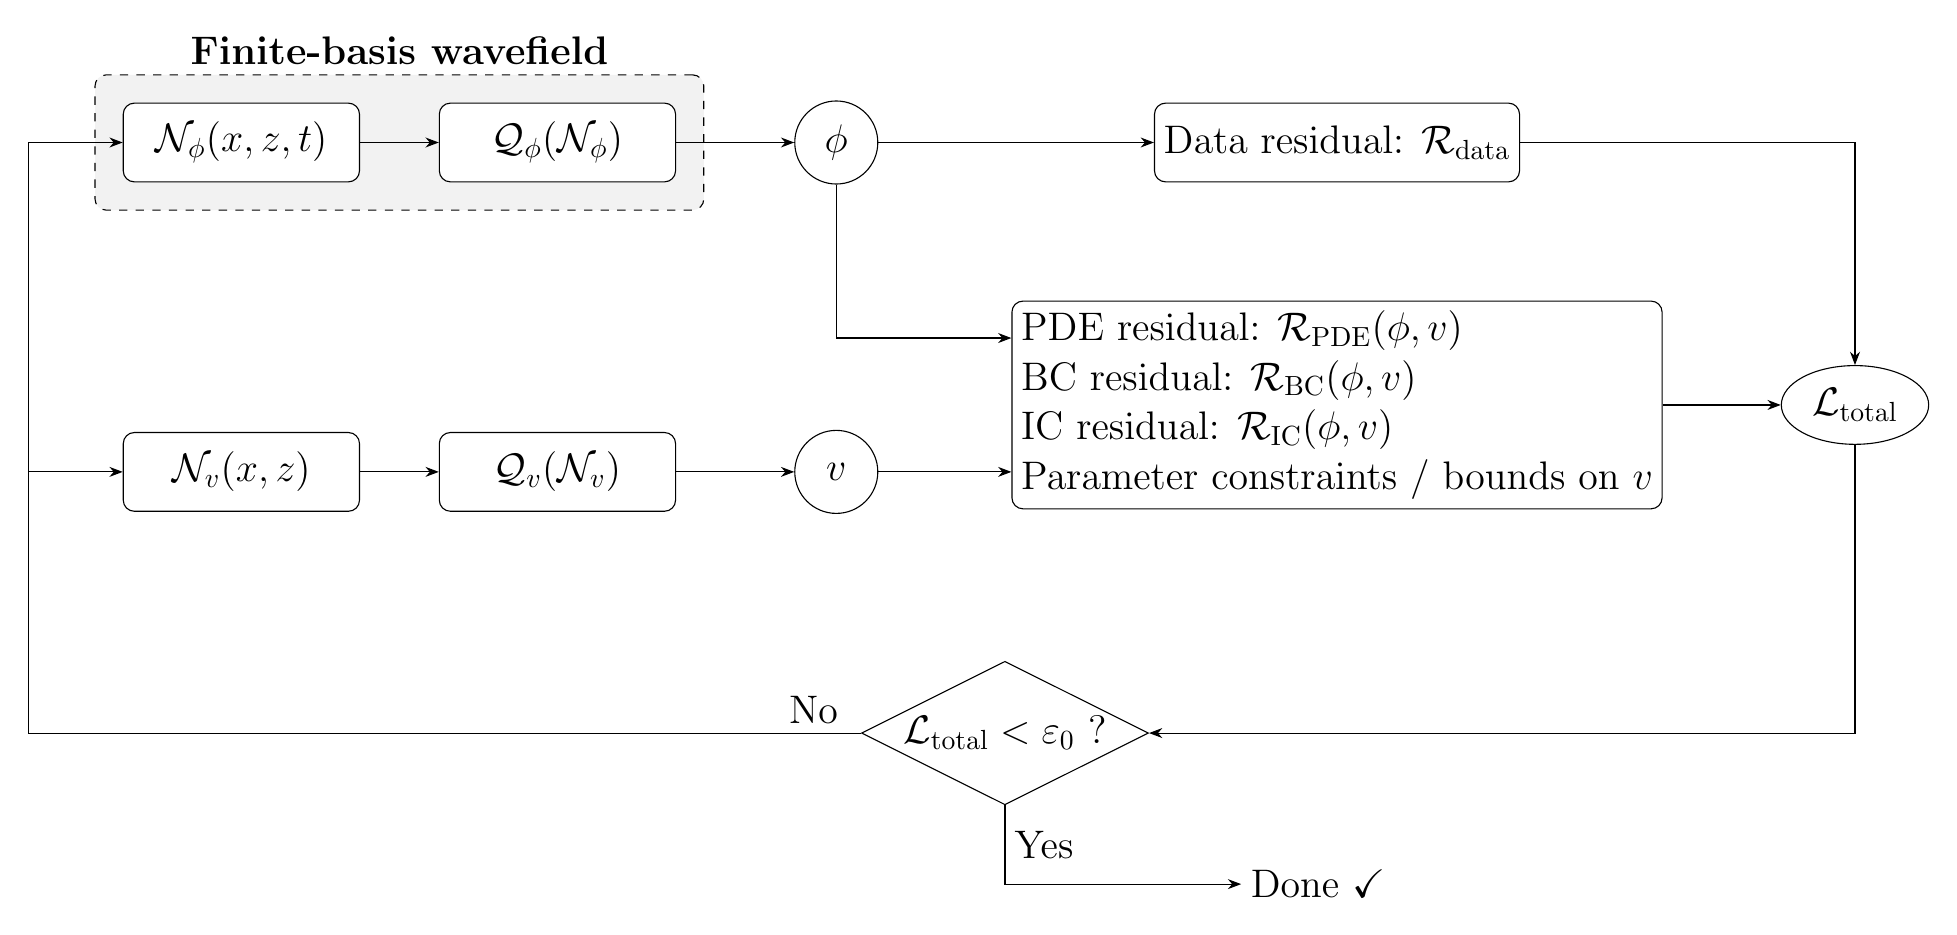
\begin{tikzpicture}[
  >=Stealth,
  font=\Large,
  node distance=2.2cm and 2.4cm,
  box/.style={draw, rounded corners, minimum width=3.0cm, minimum height=1.0cm, align=center, fill=white},
  qbox/.style={box},
  circ/.style={circle, draw, minimum size=30, fill=white},
  loss/.style={ellipse, draw, minimum width=1.8cm, minimum height=1.0cm, align=center, fill=white},
  data/.style={box, minimum width=3.0cm},
  physmain/.style={draw, rounded corners, minimum width=4.0cm, minimum height=2.0cm, align=left, fill=white},
  decision/.style={diamond, draw, aspect=2, minimum width=1.6cm, inner sep=1pt, align=center, fill=white}
]

% --- NODES ---
\node[box] (net1) {$\mathcal{N}_\phi(x, z, t)$};
\node[qbox, right=1.cm of net1] (qc1) {$\mathcal{Q}_\phi(\mathcal{N}_\phi)$};
\node[circ, right=1.5cm of qc1] (phi) {$\phi$};

\node[data, right=3.5 cm of phi] (data) {Data residual: $\mathcal{R}_{\mathrm{data}}$};
\node[physmain, below=1.5cm of data] (phys)
{PDE residual: $\mathcal{R}_{\mathrm{PDE}}(\phi,v)$\\
BC residual: $\mathcal{R}_{\mathrm{BC}}(\phi,v)$\\
IC residual: $\mathcal{R}_{\mathrm{IC}}(\phi,v)$\\
Parameter constraints / bounds on $v$};
\node[loss, right=1.5cm of phys] (loss) {$\mathcal{L}_{\mathrm{total}}$};

\coordinate (phys_lower) at ([yshift=-0.85cm]phys.center);
\node[box] (net2) at (net1 |- phys_lower) {$\mathcal{N}_v(x,z)$};
\node[qbox, right=1.cm of net2] (qc2) {$\mathcal{Q}_v(\mathcal{N}_v)$};
\node[circ, right=1.5cm of qc2] (cvar) {$v$};

% --- BACKGROUND BOX ---
\begin{scope}[on background layer]
    % Invisible bounding box to maintain layout alignment for later nodes
    \node[inner sep=15pt, fit=(net1) (net2) (qc1) (qc2)] (hybridbox) {};
    
    % Wavefield box
    \node[draw, dashed, fill=gray!10, rounded corners, inner sep=10pt, 
          fit=(net1) (qc1), label={[yshift=0.0cm]above:\textbf{Finite-basis wavefield}}] (wavebox) {};
\end{scope}

% --- CENTERED DECISION NODE ---
% This calculates the horizontal center between the hybridbox west and loss east
\node[decision] (eps) at ($(hybridbox.west |- 0, -7.5) !0.5! (loss.east |- 0, -7.5)$) {$\mathcal{L}_{\mathrm{total}} < \varepsilon_0$ ?};

% --- CONNECTIONS ---
\draw[->] (net1) -- (qc1);
\draw[->] (net2) -- (qc2);
\draw[->] (qc1) -- (phi);
\draw[->] (qc2) -- (cvar);
\draw[->] (phi) -- (data.west);
\draw[->] (phi) |- ([yshift=0.85cm]phys.west);
\draw[->] (cvar) -- (cvar -| phys.west);
\draw[->] (data.east) -| (loss.north);
\draw[->] (phys.east) -- (loss.west);

% Path to loss
\draw[->] (loss.south) |- (eps.east);

% Feedback loop
\draw[-] (eps.west) -- node[above, pos=0.2] {No} ++(-3cm,0) -| ([xshift=-1.2cm]net2.west);
\draw[->] ([xshift=-1.2cm]net2.west) |- (net1.west);
\draw[->] ([xshift=-1.2cm]net2.west) -- (net2.west);

% Yes path: Down, then Right
\draw[->] (eps.south) |- ++(3cm, -1.0cm) node[right] {Done \checkmark} 
    node[near start, right] {Yes};

\end{tikzpicture}%
}
\caption{Schematic of the finite-basis classical-quantum hybrid architecture, combining classical neural networks and quantum circuits with physics-informed constraints. $\mathcal{N}$ denotes classical networks, $\mathcal{Q}$ quantum circuits, $\phi$ the predicted wavefield, $v$ the inverted velocity, and $\mathcal{R}$ the physics- and data-based residuals.}
\label{fig:hybrid_arch}
\end{figure}

\def\myvdots{\ \vdots\ }
\def\myddots{\ \ddots\ }
\begin{figure}[h]
\centering
\resizebox{0.9\linewidth}{!}{
    \begin{quantikz}
    \lstick{$\ket{q_1}$}
        & \gate{R_y(\beta_1 z_1)}
            \gategroup[5,steps=1,style={dashed, fill=gray!10, rounded corners, inner xsep=2pt},background,
            label style={label position=below,anchor=north,yshift=-0.2cm}]
            {{\textbf{Encoding}}}
        & \gate{R_x(\theta_{1,2})}
            \gategroup[5,steps=7,style={dashed, fill=gray!10, rounded corners, inner xsep=2pt},background,
            label style={label position=below,anchor=north,yshift=-0.2cm}]
            {{\textbf{Repeat $L$ times}}}
        & \gate{R_y(\theta_{1,3})}
        & \gate{R_z(\theta_{1,4})}
        & \ctrl{1} & & & & \meter{} \\
    \lstick{$\ket{q_2}$}
        & \gate{R_y(\beta_2 z_2)}
        & \gate{R_x(\theta_{2,2})}
        & \gate{R_y(\theta_{2,3})}
        & \gate{R_z(\theta_{2,4})}
        & \targ{} 
        & \ctrl{1} & & & \meter{}\\
    \lstick{$\ket{q_3}$}
        & \gate{R_y(\beta_3 z_3)}
        & \gate{R_x(\theta_{3,2})}
        & \gate{R_y(\theta_{3,3})}
        & \gate{R_z(\theta_{3,4})}
        & & \targ{}
        & \ctrl{1}
        & & \meter{} \\
    \setwiretype{n} \myvdots
        & \myvdots & \myvdots & \myvdots & \myvdots
        & \myvdots & \myvdots & \myddots & \myddots & \myvdots \\
    \lstick{$\ket{q_n}$}
        & \gate{R_y(\beta_n z_n)}
        & \gate{R_x(\theta_{n,2})}
        & \gate{R_y(\theta_{n,3})}
        & \gate{R_z(\theta_{n,4})}
        & & & & \targ{} & \meter{}
    \end{quantikz}
}
\caption{Multilayer PQC $\mathcal{Q}$. Each input feature $z_i$ is angle-encoded via an $R_y(\beta_i\, z_i)$ rotation (encoding layer, grey), where $\beta_i$ is a trainable scaling parameter. Variational layers of single-qubit rotations $R_x$, $R_y$, $R_z$ followed by a linear CNOT ladder are repeated $L$ times (grey block). Each qubit is measured in the Pauli-$Z$ basis, and the outputs are averaged to yield a scalar in $[-1, 1]$.}
\label{fig:pqc_architecture}
\end{figure}


\begin{table}[h]
\centering
\caption{Network configurations for the anomaly benchmark. $\mathcal{Q}(n_q^{\times n_L})$ denotes a PQC with $n_q$ qubits and $n_L$ layers. Subdomain decomposition ($5\!\times\!3\!\times\!5$, overlap 0.35) applies to the wavefield network $\phi$; the velocity network $v$ is a single global network. Loss weights: $\lambda_\text{PDE}\!=\!0.1$, $\lambda_\text{IC}\!=\!1.0$, $\lambda_\text{data}\!=\!1.0$, $\lambda_\text{BC}\!=\!0.1$. Learning rate $10^{-4}$. See Supplementary Table~S1 for the full hyperparameter variant sweep.}
\label{tab:hyperparams_main}
\begin{tabular}{l l l r}
\toprule
\textbf{Model} & \makecell[l]{$\boldsymbol{\phi}$ \textbf{network}\\$(x,z,t)\!\to\!\phi$} & \makecell[l]{$\boldsymbol{v}$ \textbf{network}\\$(x,z)\!\to\!v$} & \textbf{\# Params} \\
\midrule
\texttt{classical} & $\mathcal{N}\!: 32^{\times 2}\!\to\!16^{\times 2}$ & $\mathcal{N}\!: 20^{\times 5}$ & 151{,}836 \\
\texttt{quantum}   & $\mathcal{N}\!: 32^{\times 2}\!\to\!\mathcal{Q}\!: 4^{\times 2}$ & $\mathcal{N}\!: 20^{\times 3}\!\to\!\mathcal{Q}\!: 4^{\times 2}$ & 101{,}812 \\
\bottomrule
\end{tabular}
\end{table}

\subsection{Anomaly benchmark}
\label{sec:results_anomaly}

Our primary evaluation uses the velocity model established by Rasht-Behesht et al.~\cite{rahst}, which defines a 2D acoustic domain ($1.15$\,km\,$\times$\,$0.45$\,km) featuring a localized low-velocity anomaly ($\sim$$2.5$\,km/s embedded within a $\sim$$3.0$\,km/s background; Figure~\ref{fig:anomaly}a). Ground-truth receiver data are generated with SPECFEM2D~\newcite{komatitsch1998spectral} driven by a Gaussian source at $(0.35,\,0.19)$\,km with dominant frequency $f_0 = 60$\,Hz. The inversion process is constrained by $500$\,ms of wavefield displacements recorded by a vertical array of 20 receivers positioned along the right boundary ($x = 1.15$\,km), supplemented by two early displacement snapshots ($t_0 = 0.100$\,s and $t_1 = 0.115$\,s). This transmission-dominated configuration, featuring a single source and a one-sided receiver array, represents a severely ill-posed inverse problem. The limited angular illumination inherently restricts the recovery of high-wavenumber spatial components, rigorously testing the regularizing capacity of the chosen neural architecture.

Starting from a purely homogeneous initial guess (Figure~\ref{fig:anomaly}b), both the classical and hybrid architectures successfully localize the low-velocity anomaly without suffering from the cycle-skipping artifacts that frequently plague classical adjoint-state FWI under poor starting models. As illustrated by the inverted velocity field of the quantum hybrid model (Figure~\ref{fig:anomaly}c), the recovered anomaly closely tracks the true model's spatial distribution and peak amplitude. The minor lateral smearing observed in the reconstruction is consistent with the theoretical limits of resolving power imposed by the single-source geometry, confirming that the network has extracted the maximum available information from the receiver data.

The most profound distinction between the classical and quantum approaches emerges in their optimization dynamics. Figure~\ref{fig:anomaly}d tracks the L1 velocity error against training iterations, revealing structurally different convergence trajectories. The quantum hybrid model undergoes a rapid initial descent, achieving an L1 error of $2.4\times 10^{-2}$ in merely $65{,}000$ iterations. In stark contrast, the classical baseline exhibits prolonged plateauing behavior, requiring $500{,}000$ iterations to reach a comparable, albeit slightly higher, final error of $2.9\times 10^{-2}$. This constitutes an approximate $8\times$ acceleration in the necessary optimization steps, achieved despite the hybrid model operating with a significantly lower number of trainable parameters ($101{,}812$ vs.\ $151{,}836$).

To rigorously confirm that this performance gap is fundamentally architectural rather than an artifact of sub-optimal classical tuning, we conducted an exhaustive ablation study comprising 15 distinct classical FBPINN variants. These baselines spanned a wide spectrum of configurations, including severely over-parameterized velocity networks (up to $60\!\times\!3$ hidden layers), alternative subdomain partitions ($3\!\times\!2\!\times\!3$ and $8\!\times\!4\!\times\!8$), varying learning rates, and adjusted physical loss weightings (detailed comprehensively in Supplementary Table~S1). As depicted by the thin colored traces in Figure~\ref{fig:anomaly}d, simply increasing classical capacity or tuning hyperparameters failed to bridge the gap; none of the 15 classical configurations could match the steep descent or the final L1 error of the quantum hybrid trajectory at any stage during the $500{,}000$ iterations.

\begin{figure}[H]
\centering
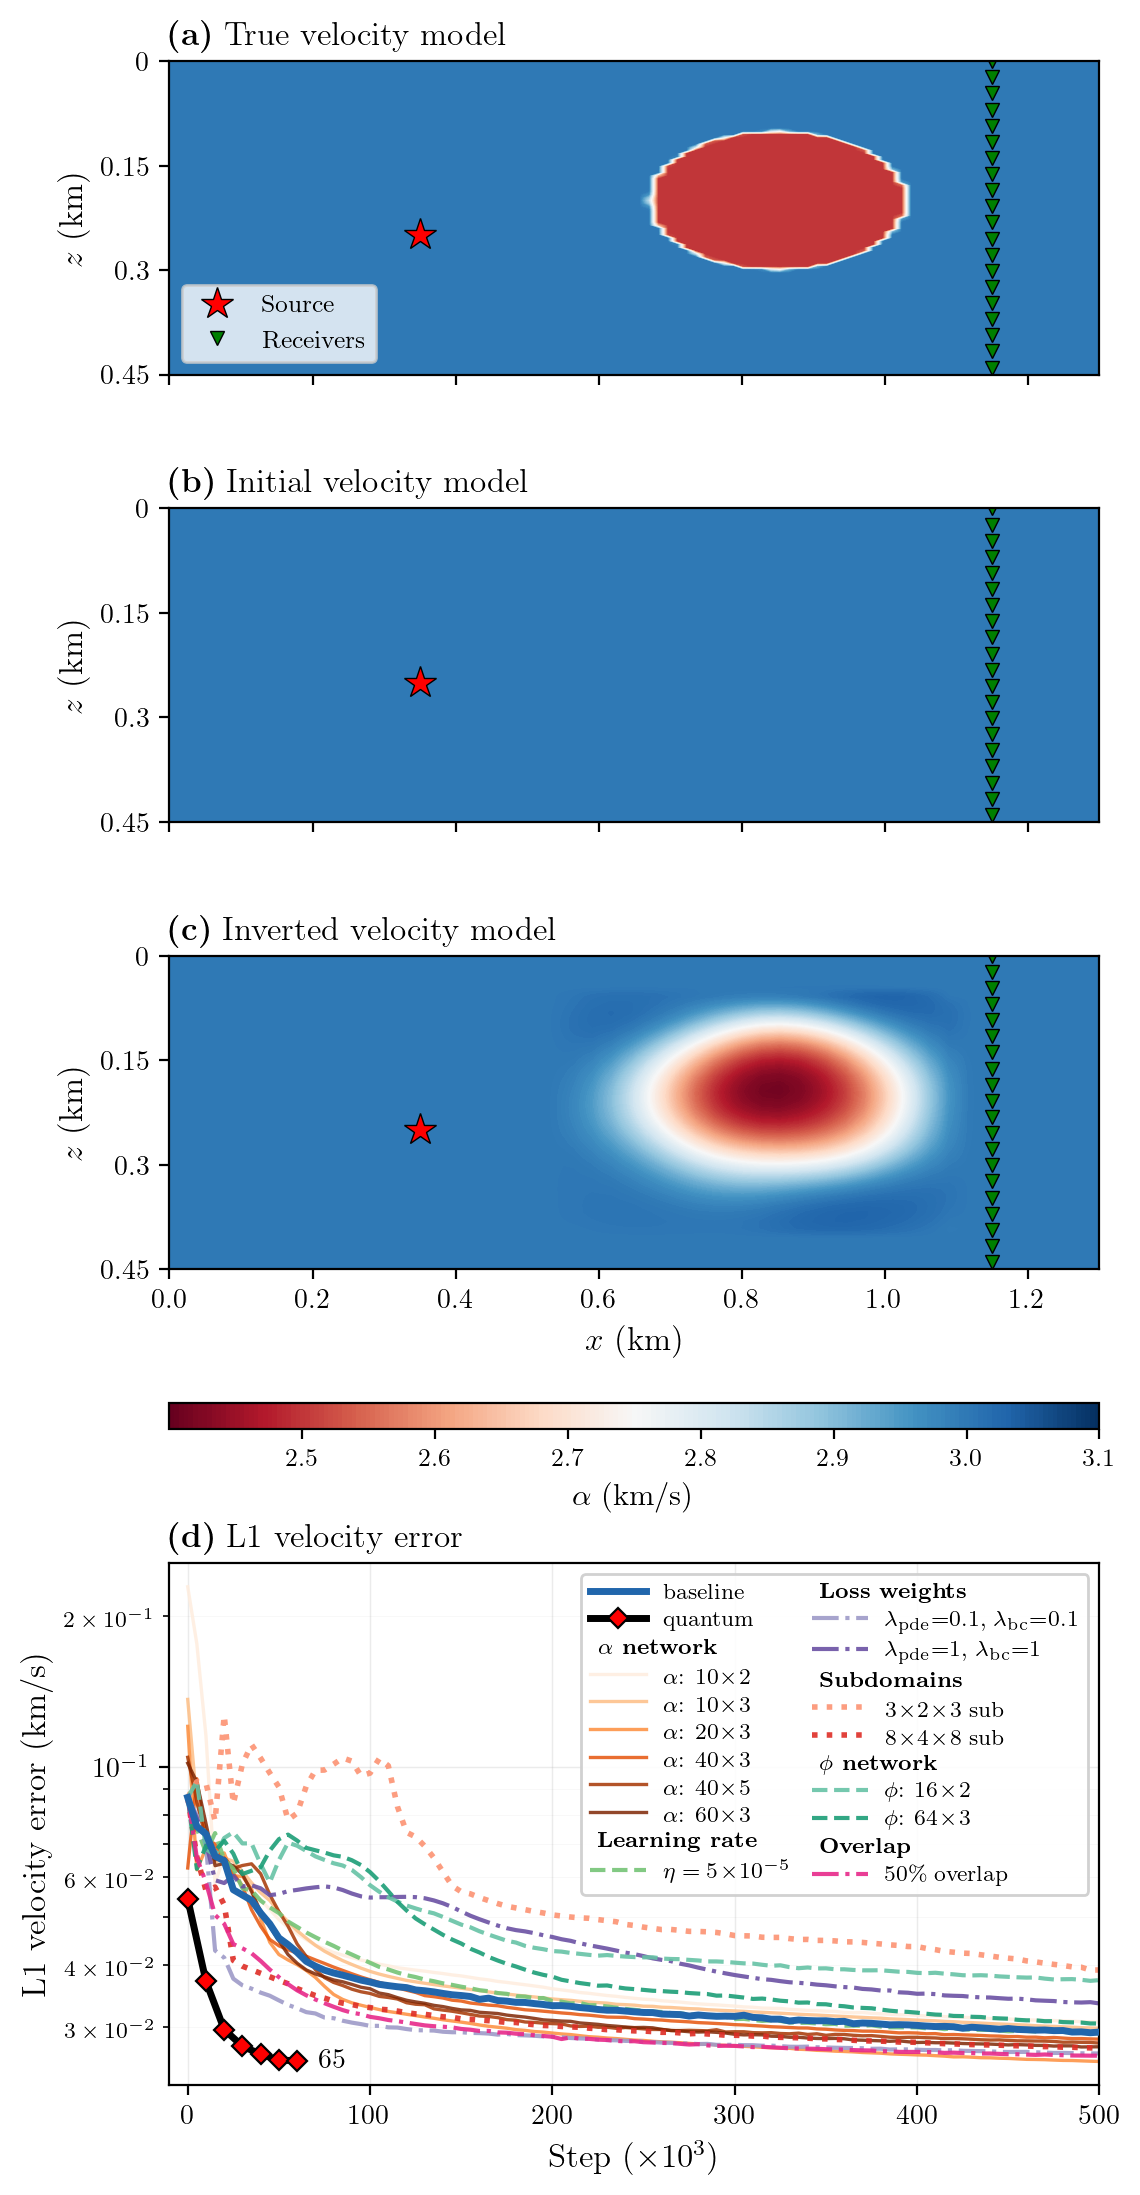
\includegraphics[width=0.6\linewidth]{../results/rasht/plots/l1_and_velocity.png}
\caption{Anomaly benchmark inversion and convergence. (a) True velocity model used for the SPECFEM2D forward simulation, with source (red star) and receiver array (green triangles). (b) Initial homogeneous velocity model. (c) Inverted velocity model from the quantum hybrid FBPINN at $65{,}000$ training iterations. (d) L1 velocity error versus training iteration for the classical FBPINN baseline (blue), the quantum hybrid (red markers labelled 65k), and 15 classical hyperparameter variants (thin coloured lines).}
\label{fig:anomaly}
\end{figure}

\subsection{Checkerboard benchmark}
\label{sec:results_checkerboard}

To further probe the resolution limits of the inversion pipeline, we test a checkerboard velocity model: a $3\times 3$ grid of alternating $\pm$$0.4$\,km/s perturbations on a $3.0$\,km/s background. The acquisition geometry is identical to the anomaly benchmark --- same domain, source position, and receiver layout (Figure~\ref{fig:anomaly}a) --- as is the homogeneous initial model (Figure~\ref{fig:anomaly}b). The checkerboard forward simulation, however, uses a lower dominant source frequency, $f_0 = 20$\,Hz, compared with $f_0 = 60$\,Hz for the anomaly benchmark.

Both the classical and quantum hybrid FBPINNs are run with the exact same network architectures and hyperparameters established for the anomaly benchmark (Table~\ref{tab:hyperparams_main}). The training setup differs only in the use of a higher collocation point density, required to adequately constrain the smaller-scale spatial structures of the checkerboard pattern. Both models successfully resolve the checkerboard (Figure~\ref{fig:checkerboard_inversion}b). As expected from the single-source, one-sided receiver geometry, structural resolution degrades for blocks situated further from the receiver array. The successful inversion under this otherwise unchanged configuration confirms that the hybrid architecture generalizes beyond the anomaly benchmark without additional tuning.

\begin{figure}[h]
\centering
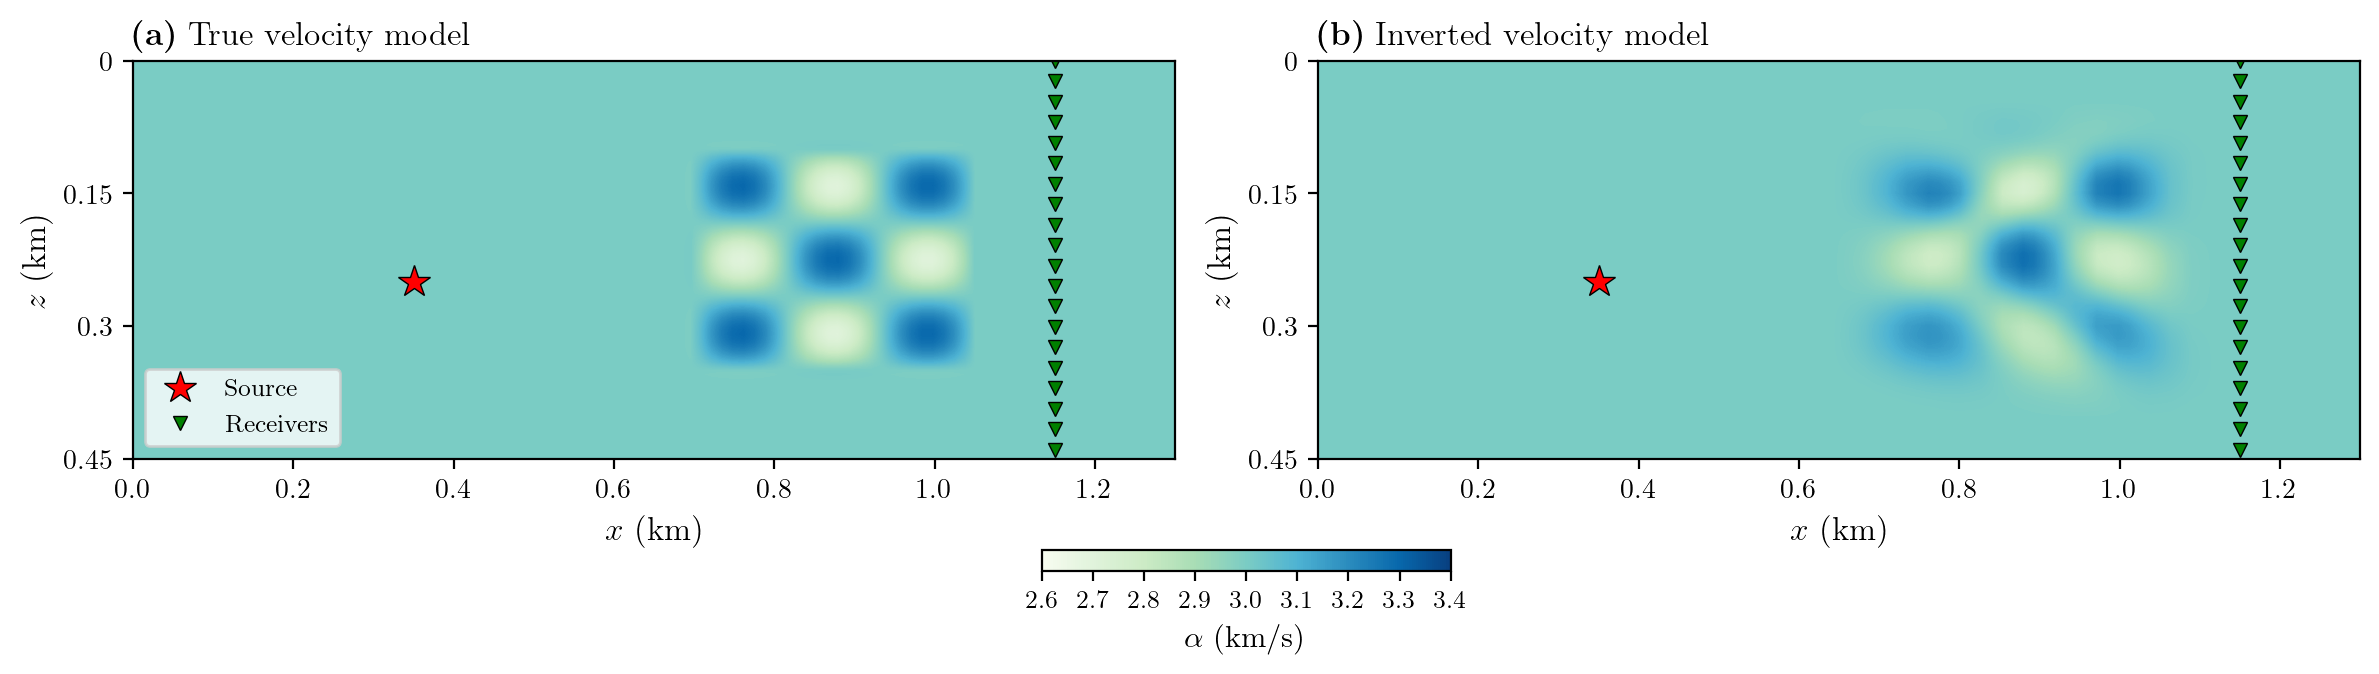
\includegraphics[width=\linewidth]{../results/checkerboard/plots/true_and_inverted.png}
\caption{Checkerboard benchmark inversion. (a) True velocity model: a $3\times 3$ checkerboard of alternating $\pm$$0.4$\,km/s perturbations on a $3.0$\,km/s background, with source (red star) and receiver array (green triangles). (b) Inverted velocity model from the quantum hybrid FBPINN, using the identical network configuration from the anomaly benchmark with only the collocation point density increased.}
\label{fig:checkerboard_inversion}
\end{figure}


\section{Discussion}\label{sec:discussion}

The quantum hybrid model reaches a lower L1 velocity error than the primary classical FBPINN baseline in approximately $8\times$ fewer training iterations, despite using $\sim$$33$\% fewer trainable parameters. Furthermore, it outperforms all 15 alternative classical hyperparameter variants tested across a wide range of parameter counts. We attribute this to three properties of the classical-to-PQC pipeline~\newcite{cerezo2021variational}. First, despite its smaller parameter count, the PQC operates on states in an exponentially large Hilbert space~\newcite{havlicek2019supervised,huang2021power}: an $n$-qubit statevector lives in $\mathbb{C}^{2^n}$ (for $n=4$, a $16$-dimensional complex space), and the measured expectation value
\begin{equation}
    f(\mathbf{x};\boldsymbol{\beta},\boldsymbol{\theta}_q) = \frac{1}{n}\sum_{i=0}^{n-1} \langle\psi(\mathbf{z}(\mathbf{x});\boldsymbol{\beta},\boldsymbol{\theta}_q)|\,Z_i\,|\psi(\mathbf{z}(\mathbf{x});\boldsymbol{\beta},\boldsymbol{\theta}_q)\rangle
\end{equation}
is a nonlinear function of all variational angles acting jointly on this high-dimensional representation. A classical multilayer perceptron (MLP) with a comparable parameter count operates in a much smaller latent space and must spend its parameters on both feature construction and output generation. Second, angle encoding endows the PQC output with a specific finite-frequency Fourier structure in the variables presented to the encoder~\newcite{schuld2021effect}. In our hybrid architecture the PQC acts on the latent vector $\mathbf{z}(\mathbf{x}) = \mathcal{N}(\mathbf{x})$ rather than directly on the spatial coordinates, so the precise statement is the corresponding specialization of the general Fourier result of \citet{schuld2021effect}:
\begin{equation}
    f(\mathbf{x};\boldsymbol{\beta},\boldsymbol{\theta}_q) = \sum_{\boldsymbol{\omega}\in\Omega} c_{\boldsymbol{\omega}}(\boldsymbol{\theta}_q)\, e^{i\,\boldsymbol{\omega}\cdot(\boldsymbol{\beta}\odot\mathbf{z}(\mathbf{x}))},
\end{equation}
where the coefficients $c_{\boldsymbol{\omega}}$ depend on the trainable circuit angles while the accessible frequency set $\Omega$ is fixed by the encoding generators and encoding pattern. To see this, for one encoded scalar $s$ with generator $G$ and encoding unitary $U_{\mathrm{enc}}(s)=e^{-i\beta s G}$, the measured PQC output can be written as
\begin{equation}
    f(s)=\langle\psi_0|\,U_{\mathrm{enc}}(s)^\dagger M(\boldsymbol{\theta}_q)\,U_{\mathrm{enc}}(s)\,|\psi_0\rangle,
\end{equation}
where $M(\boldsymbol{\theta}_q)=V(\boldsymbol{\theta}_q)^\dagger O\,V(\boldsymbol{\theta}_q)$, $V(\boldsymbol{\theta}_q)$ denotes the variational part of the circuit, and $O=\frac{1}{n}\sum_{i=0}^{n-1} Z_i$ is the measurement observable. If $G=\sum_a \lambda_a \Pi_a$ is the spectral decomposition of the encoding generator, then
\begin{equation}
    f(s)=\sum_{a,b} e^{i\beta s(\lambda_a-\lambda_b)}
    \langle\psi_0|\,\Pi_a M(\boldsymbol{\theta}_q)\Pi_b\,|\psi_0\rangle,
\end{equation}
so the accessible frequency indices are the pairwise eigenvalue differences $\Omega \subseteq \{\lambda_a-\lambda_b\}$. For the present $R_y(\beta_i z_i)$ angle encoding, $G=Y/2$ has eigenvalues $\pm\tfrac{1}{2}$, hence each coordinate contributes only indices $0,\pm 1$, corresponding to actual frequencies $0,\pm\beta_i$ in the variable $z_i$, and, for a single encoded variable,
\begin{equation}
    f(s)=A+B\cos(\beta s)+C\sin(\beta s).
\end{equation}
The trainable circuit angles can change the coefficients $A,B,C$ (and, in the multivariate setting, the coefficients $c_{\boldsymbol{\omega}}$), but they cannot create frequencies outside this accessible set. This built-in spectral prior in the PQC latent variables may match smooth, spatially-correlated velocity fields more efficiently than an unconstrained tanh MLP, which has no such structure by default. Third, the final output map hard-codes the velocity-range constraint: because $v(x,z)=v_\text{bg}+A\,\tanh(g(x,z))\,m(x,z)$ with $m(x,z)\in[0,1]$, it follows that $|v(x,z)-v_\text{bg}|\leq A\,m(x,z)\leq A$. The bounded PQC output therefore supplies a bounded latent signal before this final map, which may reduce large early-training excursions; entangling CNOT gates additionally introduce non-separable correlations between the spatial inputs that a classical MLP can only approximate through successive layers of additive linear combinations and pointwise nonlinearities. The robustness of the advantage across classical hyperparameter choices (Figure~\ref{fig:anomaly}d) argues against an unlucky baseline, though we emphasize that these gains are in optimization iterations on classically-simulated circuits and do not constitute a quantum computational advantage.

Our work complements recent hybrid quantum-PINN studies in other PDE-constrained settings. Leong et al.~\cite{LEONG2025106782} benchmarked hybrid quantum PINNs for high-speed compressible flow, finding competitive accuracy at reduced parameter cost compared with classical PINNs. Berger et al.~\cite{Berger2025} introduced trainable-embedding quantum PINNs for nonlinear PDEs including the Navier-Stokes equations, again observing efficiency gains at matched parameter count. The present work differs in two ways. First, we target a coupled forward-inverse problem (waveform inversion) rather than a pure forward PDE; the velocity field is learned jointly with the wavefield. Second, we integrate the PQC within a domain-decomposed FBPINN~\cite{Moseley2023}, extending the PINN-based FWI formulation of Rasht-Behesht et al.~\cite{rahst} to handle larger and higher-frequency inversion problems via overlapping subdomain networks.

Several limitations should be noted. (i) The present experiments are two-dimensional and acoustic. Extending to three-dimensional elastic inversion is the natural next step but is constrained by the $\mathcal{O}(2^n)$ memory cost of statevector simulation as qubit counts grow. Scaling to larger circuits on real hardware further raises the concern of barren plateaus --- vanishingly small gradients in high-depth parameterized circuits~\newcite{mcclean2018barren}, which would require careful initialization and ansatz choice. (ii) Inversions use a single source; production FWI pipelines incorporate tens to thousands of sources with different illuminations, and PINN-based FWI in particular is known to be sensitive to loss-landscape pathologies under data sparsity~\newcite{krishnapriyan2021failure}. (iii) The quantum circuit is simulated classically. On real NISQ hardware, gradients would be computed via the parameter-shift rule (two circuit evaluations per parameter), and device noise could erode the iteration-level advantage observed here.

Looking forward, the small qubit counts used here ($n=4$, $L=2$) are compatible with near-term quantum hardware, which suggests that genuine hardware demonstrations are feasible once noise-mitigation techniques reach sufficient maturity. Systematic studies at matched parameter counts across circuit depths and widths would clarify how the convergence advantage scales with quantum-circuit capacity. Because the framework targets the general structure of physics-informed wave inversion rather than any geophysics-specific feature, we expect it to transfer directly to the broader wave-based inverse problems discussed in the Introduction, including medical ultrasound tomography, photoacoustic imaging, and non-destructive evaluation.

\section{Methods}\label{sec:method}

\subsection{Acoustic wave equation}
\label{sec:methods_wave}

We consider two-dimensional acoustic wave propagation in a heterogeneous medium with spatially varying wave speed $v(\mathbf{x})$ and constant density. With no explicit source injection, the governing equation is the source-free acoustic wave equation,
\begin{equation}
\frac{\partial^{2} u(\mathbf{x},t)}{\partial t^{2}}
= v^{2}(\mathbf{x})\,\nabla^{2} u(\mathbf{x},t),
\label{eq:acoustic_wave}
\end{equation}
where $u(\mathbf{x},t)$ is a scalar potential whose spatial derivatives $(\partial u/\partial x,\, \partial u/\partial z)$ give the two components of the displacement field. Wave propagation is initiated by prescribing the wavefield at two closely spaced instants, $t_0 = 0.100$\,s and $t_1 = 0.115$\,s, using snapshots of the displacement field taken from a spectral-element simulation; both snapshots are imposed as soft constraints in the loss function. A free-stress boundary condition (vanishing acoustic pressure, equivalently $\nabla^2 u = 0$ in this displacement-potential formulation) is enforced on the top surface of the physical domain. This formulation provides a well-posed initial-boundary-value problem without requiring an explicit source time function.

\subsection{Finite-basis physics-informed neural network}
\label{sec:methods_fbpinn}

PINNs~\cite{RAISSI2019686} approximate solutions of PDEs by a neural network $u_\theta(\mathbf{x})$ and train $\theta$ to minimize the PDE residual at a set of collocation points $\{\mathbf{x}_i\}_{i=1}^{N}$ drawn from the domain. Writing the governing PDE in residual form $\mathcal{N}[u](\mathbf{x}) = 0$, the PDE loss is
\begin{equation}
    \mathcal{L}_\text{PDE}
    = \frac{1}{N} \sum_{i=1}^{N}
    \left| \mathcal{N}[u_\theta(\mathbf{x}_i)] \right|^{2},
\end{equation}
with spatial and temporal derivatives computed by automatic differentiation of the network with respect to its inputs. Boundary conditions, initial conditions, and observational data are added as additional weighted loss terms (the full composite loss used for FWI is given in the Hybrid architecture subsection below). Standard PINNs, however, are known to suffer from spectral bias, a tendency to learn low-frequency features before high-frequency ones, which severely limits their effectiveness in multi-scale wave problems such as FWI, where both the velocity field and the wavefield exhibit sharp transitions and oscillatory structure.

To overcome this limitation, we adopt the FBPINN framework of \citet{Moseley2023}. The global domain $\Omega$ is partitioned into $K$ overlapping rectangular subdomains $\{\Omega_k\}$, each equipped with an independent neural network $u_{\theta_k}(\mathbf{x})$. The global solution is reconstructed as a partition-of-unity sum,
\begin{equation}
    u(\mathbf{x}) = \sum_{k=1}^{K} w_k(\mathbf{x})\, u_{\theta_k}(\mathbf{x}),
\end{equation}
where the window functions $w_k$ are smooth cosine bumps supported on $\Omega_k$ with $\sum_k w_k(\mathbf{x}) = 1$ for all $\mathbf{x} \in \Omega$. Each local network only needs to represent the solution's behaviour on its own subdomain, with two consequences: (i) the local frequency content each network must learn is bounded by the subdomain size, alleviating spectral bias; and (ii) training is embarrassingly parallel across subdomains, enabling batched evaluation via JAX's \texttt{vmap}. The physics-informed loss is evaluated on the reconstructed global solution, so gradients flow through the window-weighted sum back to the individual subdomain networks.

For the wavefield $\phi(x,z,t)$ we use a three-dimensional subdomain decomposition $(n_x, n_z, n_t)$, $5\!\times\!3\!\times\!5$ in the anomaly baseline with subdomain overlap $0.35$. The velocity network $v(x,z)$ is not decomposed; it is a single global network, since the velocity field typically varies more smoothly than the wavefield and does not require local representation.

\subsection{Parameterized quantum circuits}
\label{sec:methods_pqc}

Basic background on qubits, quantum states, and gates is provided in the Supplementary Information. Here we use only the quantum ingredients required by the hybrid architecture. An $n$-qubit register is represented by a normalized statevector in $\mathbb{C}^{2^n}$. The circuit uses parameterized single-qubit rotations
\begin{equation}
  R_k(\theta) = e^{-i\theta\,\sigma_k/2}, \qquad k \in \{x,y,z\},
\end{equation}
where $\sigma_k$ are the Pauli matrices, together with controlled-NOT (CNOT) gates to introduce entanglement between neighbouring qubits.

\subsubsection{PQC ansatz}
\label{sec:circuit_architecture}

A PQC~\cite{benedetti2019parameterized}, also referred to as a VQC, applies a trainable unitary $U(\boldsymbol{\theta}_q)$ to the initial state $|0\rangle^{\otimes n}$ and returns a scalar expectation value of a Hermitian observable, yielding a smooth, differentiable function of the circuit parameters $\boldsymbol{\theta}_q$. Its expressibility depends on the circuit depth, qubit connectivity, and gate set~\cite{sim2019expressibility}.

The PQC employed in this work (Fig.~\ref{fig:pqc_architecture}) operates on $n$ qubits with $L$ variational layers and consists of three stages:

\begin{enumerate}
  \item \emph{Data embedding layer.} Starting from $|0\rangle^{\otimes n}$, each qubit $i$ receives an $R_y(\beta_i\, z_i)$ rotation (angle encoding~\cite{schuld2021machine}) that encodes the $i$-th component of the input vector $\mathbf{z} \in \mathbb{R}^n$, scaled by a trainable basis parameter $\beta_i$:
    \begin{equation}
      |\psi_\mathrm{enc}(\mathbf{z};\boldsymbol{\beta})\rangle = \bigotimes_{i=0}^{n-1} R_y(\beta_i\, z_i)\,|0\rangle.
    \end{equation}

  \item \emph{Variational layers.} Each of $L$ layers $l = 1, \ldots, L$ applies (i) a general single-qubit rotation $R_z(\theta^{(3)}_{l,i})\, R_y(\theta^{(2)}_{l,i})\, R_x(\theta^{(1)}_{l,i})$ to every qubit $i$, introducing $3n$ trainable parameters per layer, followed by (ii) a linear CNOT ladder $\text{CNOT}(i, i{+}1)$ for $i = 0, \ldots, n{-}2$ entangling neighbouring qubits. The total number of trainable gate parameters is $3nL$, plus $n$ basis parameters from the embedding layer.

  \item \emph{Measurement layer.} The Pauli-$Z$ expectation values $\langle Z_i \rangle$ on each qubit are averaged to produce a single scalar output
    \begin{equation}
      f(\mathbf{z}; \boldsymbol{\beta}, \boldsymbol{\theta}_q)
      = \frac{1}{n} \sum_{i=0}^{n-1} \langle\psi(\mathbf{z}; \boldsymbol{\beta}, \boldsymbol{\theta}_q)|\, Z_i \,|\psi(\mathbf{z}; \boldsymbol{\beta}, \boldsymbol{\theta}_q)\rangle
      \;\in [-1,\, 1].
      \label{eq:pqc_output}
    \end{equation}
\end{enumerate}

\subsection{JAX-based statevector simulator}
\label{sec:methods_statevector}

We implement the PQC as a lightweight statevector simulator in JAX~\citep{jax2018github} rather than relying on an external framework such as PennyLane~\citep{bergholm2022pennylaneautomaticdifferentiationhybrid} or Qiskit~\citep{javadiabhari2024quantumcomputingqiskit}. The simulator represents the quantum state as a $2^n$-dimensional complex vector and applies gate operations via tensor contractions: single-qubit rotation gates ($R_x$, $R_y$, $R_z$) are constructed as $2\!\times\!2$ unitary matrices and applied with \texttt{jnp.tensordot} on the reshaped state tensor, and CNOT gates are realised through index permutation and conditional flipping on the control-target subspace. Expectation values are computed analytically from the statevector amplitudes, without stochastic sampling, as in PennyLane's \texttt{default.qubit} backend.

On near-term quantum hardware, gradients of PQC outputs with respect to gate parameters are typically computed via the parameter-shift rule~\newcite{mitarai2018quantum,schuld2019evaluating}, which evaluates the circuit at two shifted parameter values per gate and therefore requires $2p$ circuit evaluations per gradient for a circuit with $p$ parameters. In classical statevector simulation, each gate application is already a standard differentiable operation, so embedding the circuit in JAX offers two concrete advantages. First, \texttt{jax.grad} and \texttt{jax.jvp} backpropagate through the full hybrid pipeline (classical PINN layers, quantum circuit, and loss function) without parameter-shift rules or cross-framework bridging. Second, the entire training loop can be compiled into a single optimized XLA program via \texttt{jax.jit}, eliminating Python-level dispatch and framework-bridging overhead. The trade-off is that statevector simulation scales as $\mathcal{O}(2^n)$ in memory and $\mathcal{O}(L\,n\,2^n)$ in computation, limiting the approach to moderate qubit counts; for the circuit sizes used here ($n \leq 8$, $L \leq 6$), this cost is negligible compared with the classical network and loss evaluation. We verify numerical correctness by comparing parameter gradients $\partial f/\partial\boldsymbol{\theta}_q$ against PennyLane's \texttt{default.qubit} backend~\newcite{bergholm2018pennylane} across eight circuit configurations (2-8 qubits, 1-6 layers); the maximum absolute deviation is below $2\times 10^{-7}$, consistent with \texttt{float32} machine precision (Supplementary Fig.~S1).

\subsection{Hybrid quantum-classical architecture}\label{sec:hybrid_network}

The hybrid architecture (Figure~\ref{fig:hybrid_arch}) couples two neural networks with physics-informed constraints: a wavefield network $\phi(x,z,t)$, decomposed across subdomains as described in \S\ref{sec:methods_fbpinn}, and a velocity network $v(x,z)$, which is a single global network. In the classical baseline, both networks are fully-connected tanh networks. In the quantum hybrid, both networks are classical-to-quantum pipelines.

Defining the latent vector
\begin{equation}
    \mathbf{z}(\mathbf{x}) = \mathcal{N}(\mathbf{x}; \boldsymbol{\theta}_c),
\end{equation}
each classical-to-quantum pipeline has the form
\begin{equation}
    g(\mathbf{x}) = w_\text{out}\, \mathcal{Q}\!\left(\mathbf{z}(\mathbf{x}); \boldsymbol{\beta}, \boldsymbol{\theta}_q\right) + b_\text{out},
\end{equation}
where $\mathcal{N}(\mathbf{x}; \boldsymbol{\theta}_c)$ is a classical fully-connected tanh sub-network with parameters $\boldsymbol{\theta}_c$, $\mathcal{Q}(\cdot; \boldsymbol{\beta}, \boldsymbol{\theta}_q)$ is the PQC of \S\ref{sec:methods_pqc} with encoding scales $\boldsymbol{\beta}$ and variational circuit parameters $\boldsymbol{\theta}_q$ (returning a scalar in $[-1,1]$), and $(w_\text{out}, b_\text{out})$ are learnable output weights. For the anomaly benchmark experiments we use $n = 4$ qubits and $L = 2$ variational layers in both networks. The velocity network output is further mapped to physical velocity units via
\begin{equation}
    v(x,z) = v_\text{bg} + A\, \tanh\!\big(g(x,z)\big) \cdot m(x,z),
    \label{eq:velocity_output}
\end{equation}
with background velocity $v_\text{bg} = 3.0$\,km/s, amplitude $A = 2.0$\,km/s, and a smooth spatial mask $m(x,z) \in [0,1]$ (the product of four logistic cutoffs) that confines the velocity perturbation to the interior of the physical domain. This construction hard-codes physical bounds ($|v - v_\text{bg}| \leq A$) and zero perturbation at the domain edges, acting as a mild regularization of the inverse problem.

The full training objective is
\begin{equation}
\mathcal{L}_\text{total}
= \lambda_\text{data}\,\mathcal{L}_\text{data}(\phi)
+ \lambda_\text{PDE}\,\mathcal{L}_\text{PDE}(\phi, v)
+ \lambda_\text{BC}\,\mathcal{L}_\text{BC}(\phi)
+ \lambda_\text{IC}\,\mathcal{L}_\text{IC}(\phi),
\end{equation}
where $\mathcal{L}_\text{data}$ is the data misfit between the predicted and observed displacement fields at the receiver locations, $\mathcal{L}_\text{PDE}$ enforces the source-free acoustic wave equation~(\ref{eq:acoustic_wave}) via automatic differentiation, and $\mathcal{L}_\text{IC}, \mathcal{L}_\text{BC}$ are the snapshot-based initial-condition and free-stress boundary-condition constraints. All parameters (classical-network weights $\boldsymbol{\theta}_c$, embedding scales $\boldsymbol{\beta}$, variational circuit angles $\boldsymbol{\theta}_q$, and output scalings) are optimized jointly by Adam gradient descent through the full differentiable pipeline.

\subsection{Training setup}
\label{sec:methods_training}

All training uses the Adam optimizer at learning rate $10^{-4}$ (baseline; see Supplementary Table~S1 for variants). Each training step uses a collocation batch of shape $(n_x, n_z, n_t) = (40,40,25)$ across the subdomains ($40{,}000$ PDE collocation points in total), together with $40\!\times\!40 = 1{,}600$ points per displacement snapshot for the two initial-condition constraints, $\sim$$1{,}000$ receiver observations (20 receivers subsampled every 100 SPECFEM timesteps), and $5{,}000$ randomly sampled boundary-condition points on the top surface. The composite loss uses fixed weights $\lambda_\text{PDE} = 0.1$, $\lambda_\text{IC} = 1.0$ (applied equally to the two snapshot constraints), $\lambda_\text{data} = 1.0$ (receiver data), and $\lambda_\text{BC} = 0.1$. The classical baseline is trained for $500{,}000$ iterations; the quantum hybrid is trained for $65{,}000$ iterations, at which point it has already surpassed the classical baseline's $500{,}000$-step L1 velocity error.

Training uses JAX's \texttt{jit} and \texttt{vmap} transformations to compile the update step into a single XLA program and batch evaluation over subdomains. The complete update step (classical-network forward/backward passes, PQC statevector evolution, Jacobian computation via chained forward-mode \texttt{jvp}, and the composite loss) executes as a single GPU kernel. All experiments were performed on a single NVIDIA GeForce RTX 5090 GPU with \texttt{float64} precision. For the quantum hybrid, the statevector footprint is negligible: the 4-qubit PQC requires only $2^4 = 16$ complex amplitudes per forward pass, so memory cost is dominated by the classical wavefield subdomain networks. Synthetic receiver data and initial snapshots were generated with SPECFEM2D~\newcite{komatitsch1998spectral}, and spatial coordinates were scaled by $L_x = L_z = 3$\,km in all training computations.


\section{Conclusions}

We introduced a hybrid quantum-classical FBPINN for acoustic FWI, in which the decomposed wavefield network and the global velocity network are represented by PQC-based classical-to-quantum pipelines within a domain-decomposed physics-informed framework. The approach is implemented as an end-to-end differentiable JAX program, avoiding parameter-shift-rule overhead and enabling efficient joint optimization of classical PINN parameters and quantum circuit angles. On the anomaly benchmark, the hybrid model converges in $\sim$$8\times$ fewer training iterations than the primary classical FBPINN baseline, despite using $\sim$$33$\% fewer trainable parameters, and it outperforms all 15 alternative classical hyperparameter variants. We emphasize that these gains are in optimization iteration count on classically simulated circuits and do not constitute a claim of quantum computational advantage. Key limitations include reliance on classical statevector simulation, a two-dimensional acoustic setup, and a single-source configuration; extension to elastic, three-dimensional, and multi-source inversion, as well as validation on near-term quantum hardware, are the natural next steps. The framework generalizes beyond geophysics to any wave-based inverse problem amenable to physics-informed learning.


\section*{Data availability}
The synthetic receiver data used in this study were generated with SPECFEM2D~\newcite{komatitsch1998spectral} and are available in the project repository at \url{https://github.com/x-repos/quFWI} under \texttt{data/rasht/} and \texttt{data/checkerboard/}.

\section*{Code availability}
The JAX-based quantum simulator and \texttt{quFWI} framework presented here are available at \url{https://github.com/x-repos/quFWI}. Our implementation builds upon the FBPINNs framework~\cite{Moseley2023} (\url{https://github.com/benmoseley/FBPINNs}) with the PINN-based FWI formulation of Rasht-Behesht et al.~\cite{rahst} (\url{https://github.com/maziarash/PINN-FWI}).

\section*{Acknowledgments}
We thank the Reservoir Characterization Project (RCP), Colorado School of Mines, for financial support.

\section*{Author contributions}
% FILL: author contribution statement.

\section*{Conflicts of interest}
The authors declare no competing interests.

\bibliographystyle{unsrtnat}
\bibliography{refs}

\end{document}
